\documentclass[11pt,a4paper]{article}
\usepackage{fontspec}
\setmainfont{Times New Roman}
\setsansfont{Arial}
\setmonofont{Consolas}
\usepackage[a4paper,margin=2.0cm]{geometry}
\usepackage{xcolor}
\usepackage{tikz}
\usetikzlibrary{calc}
\usepackage{booktabs}
\usepackage{tabularx}
\usepackage{graphicx}
\usepackage{float}
\usepackage{listings}
\usepackage{hyperref}
\usepackage{fancyhdr}

\definecolor{deepblue}{RGB}{14,58,130}
\definecolor{accentblue}{RGB}{37,99,235}
\definecolor{codebg}{RGB}{247,249,252}

\setlength{\emergencystretch}{3em}
\hbadness=10000
\hfuzz=2pt

\lstdefinelanguage{SystemVerilog}{
    keywords={module,endmodule,input,output,inout,logic,signed,parameter,localparam,typedef,enum,always_ff,always_comb,posedge,negedge,or,if,else,case,endcase,default,begin,end,for,integer},
    sensitive=true,
    morecomment=[l]{//},
    morecomment=[s]{/*}{*/}
}

\lstset{
    language=SystemVerilog,
    backgroundcolor=\color{codebg},
    basicstyle=\ttfamily\scriptsize,
    keywordstyle=\color{deepblue}\bfseries,
    commentstyle=\color{gray}\itshape,
    frame=single,
    rulecolor=\color{accentblue!40},
    breaklines=true,
    breakatwhitespace=false,
    columns=fullflexible,
    keepspaces=true,
    showstringspaces=false,
    tabsize=4
}

\pagestyle{fancy}
\fancyhf{}
\fancyhead[L]{\small\textcolor{deepblue}{Báo Cáo Thực Hành Thiết Kế Số \& FPGA Autopilot}}
\fancyhead[R]{\small\texttt{adder\_sub\_7seg}}
\fancyfoot[C]{\thepage}

\begin{document}

% ==================== TIKZ BLUE DOUBLE-LINE COVER PAGE ====================
\begin{titlepage}
    \begin{tikzpicture}[remember picture, overlay]
        \draw[color=deepblue, line width=2.4pt]
            ($(current page.north west)+(1.2cm,-1.2cm)$)
            rectangle
            ($(current page.south east)+(-1.2cm,1.2cm)$);
        \draw[color=accentblue, line width=0.9pt]
            ($(current page.north west)+(1.42cm,-1.42cm)$)
            rectangle
            ($(current page.south east)+(-1.42cm,1.42cm)$);
    \end{tikzpicture}

    \centering
    \vspace*{1.6cm}
    {\Large\bfseries\textcolor{deepblue}{ĐẠI HỌC QUỐC GIA — PHÒNG THÍ NGHIỆM VI MẠCH \& FPGA}\\[0.3cm]}
    {\large\textsc{Digital Systems Design \& Quartus II Verification Lab Report}}\\[1.2cm]

    \rule{0.82\textwidth}{1.2pt}\\[0.5cm]
    {\huge\bfseries\textcolor{deepblue}{4-Bit Signed Adder/Subtractor + Dual 7-Segment Decoder}}\\[0.4cm]
    {\Large Module: \texttt{adder\_sub\_7seg}}\\[0.4cm]
    \rule{0.82\textwidth}{1.2pt}\\[1.4cm]

    \begin{tabularx}{0.84\textwidth}{@{}lX@{}}
        \toprule
        \textbf{Hạng mục (Metadata)} & \textbf{Thông số kỹ thuật (Specification)} \\
        \midrule
        Tên bài thí nghiệm (Benchmark) & \texttt{adder\_sub\_7seg} \\
        Kit FPGA mục tiêu (Target Kit) & DE2-115 (Cyclone IV E) \\
        Mã chip FPGA (Device Part) & \texttt{EP4CE115F29C7} \\
        Tần số xung nhịp (Target Clock) & 50.0 MHz \\
        Kết quả kiểm tra tĩnh (Static Lint) & PASS (0 Latches, 0 Width Warnings) \\
        Kết quả mô phỏng (Self-Checking TB) & 512 / 512 Vectors Passed (100\%) \\
        Trình tổng hợp (Synthesis Engine) & \texttt{quartus} \\
        \bottomrule
    \end{tabularx}

    \vfill
    {\normalsize Hệ thống tự động hóa thiết kế và kiểm chứng phần cứng \textbf{FPGA Autopilot}}\\[0.2cm]
    {\small Generated with 100\% Bit-Exact Simulation \& Hardware Synthesis Verification}
    \vspace*{1.2cm}
\end{titlepage}

\section{Tổng Quan Thiết Kế \& Đặc Tả Cổng Giao Tiếp (Port Specification)}
Pure combinational 4-bit two's-complement adder/subtractor with carry-out, signed overflow, zero flag, and dual active-low 7-segment display decoders for sign and magnitude on Terasic DE2-115.

\begin{table}[H]
    \centering
    \small
    \caption{Bảng đặc tả giao diện cổng vào/ra của module \texttt{adder\_sub\_7seg}}
    \begin{tabularx}{\textwidth}{@{}llllX@{}}
        \toprule
        \textbf{Port} & \textbf{Dir} & \textbf{Width} & \textbf{Type} & \textbf{Chức năng (Description)} \\
        \midrule
        \texttt{a} & input & 4 & signed & 4-bit signed operand A (-8 to +7) \\
        \texttt{b} & input & 4 & signed & 4-bit signed operand B (-8 to +7) \\
        \texttt{sub\_mode} & input & 1 & logic & Operation select (0: A + B, 1: A - B) \\
        \texttt{result} & output & 4 & signed & 4-bit two's-complement signed sum/difference \\
        \texttt{cout} & output & 1 & logic & Carry-out bit from MSB adder stage \\
        \texttt{overflow} & output & 1 & logic & Signed two's-complement arithmetic overflow flag \\
        \texttt{zero} & output & 1 & logic & Asserted high when result == 0 \\
        \texttt{seg\_sign} & output & 7 & active-low & Active-low 7-segment sign output ('-' when result < 0, blank otherwise) \\
        \texttt{seg\_mag} & output & 7 & active-low & Active-low 7-segment magnitude output (0..8) \\
        \bottomrule
    \end{tabularx}
\end{table}



\section{Triển Khai RTL SystemVerilog Chuẩn Tổng Hợp (Synthesizable RTL)}
Thiết kế tuân thủ nghiêm ngặt quy tắc SystemVerilog-2012: sử dụng \texttt{always\_ff} với phép gán không chặn (\texttt{<=}) cho mạch tuần tự, \texttt{always\_comb} với giá trị mặc định tường minh ở đầu khối cho mạch tổ hợp, cam kết \textbf{0 inferred latches}.

\begin{lstlisting}
// Auto-generated by fpga_autopilot — Strict Synthesizable SystemVerilog-2012
// Zero inferred latches, pure combinational arithmetic + dual active-low 7-seg decoder

module adder_sub_7seg (
    input  logic signed [3:0] a,
    input  logic signed [3:0] b,
    input  logic              sub_mode,
    output logic signed [3:0] result,
    output logic              cout,
    output logic              overflow,
    output logic              zero,
    output logic        [6:0] seg_sign,
    output logic        [6:0] seg_mag
);

    logic [3:0] a_u;
    logic [3:0] b_eff;
    logic [4:0] sum_ext;
    logic [3:0] mag;

    always_comb begin
        // Explicit default assignments guarantee 0 inferred latches
        a_u      = 4'd0;
        b_eff    = 4'd0;
        sum_ext  = 5'd0;
        result   = 4'sd0;
        cout     = 1'b0;
        overflow = 1'b0;
        zero     = 1'b0;
        mag      = 4'd0;
        seg_sign = 7'b111_1111;
        seg_mag  = 7'b111_1111;

        a_u      = a[3:0];
        b_eff    = b[3:0] ^ {4{sub_mode}};
        sum_ext  = {1'b0, a_u} + {1'b0, b_eff} + {4'b0000, sub_mode};

        result   = $signed(sum_ext[3:0]);
        cout     = sum_ext[4];
        overflow = (a_u[3] == b_eff[3]) && (sum_ext[3] != a_u[3]);
        zero     = (sum_ext[3:0] == 4'd0);

        if (sum_ext[3]) begin
            seg_sign = 7'b011_1111; // '-' on segment g (active-low)
            mag      = (~sum_ext[3:0]) + 4'd1;
        end else begin
            seg_sign = 7'b111_1111; // blank when >= 0 (active-low)
            mag      = sum_ext[3:0];
        end

        case (mag)
            4'h0:    seg_mag = 7'b100_0000;
            4'h1:    seg_mag = 7'b111_1001;
            4'h2:    seg_mag = 7'b010_0100;
            4'h3:    seg_mag = 7'b011_0000;
            4'h4:    seg_mag = 7'b001_1001;
            4'h5:    seg_mag = 7'b001_0010;
            4'h6:    seg_mag = 7'b000_0010;
// ... (truncated for report conciseness; full source in rtl/ directory)
\end{lstlisting}

\section{Kiểm Chứng Tự Động (Self-Checking Testbench Coverage)}
\begin{table}[H]
    \centering
    \small
    \caption{Tổng hợp kết quả Linting và Mô phỏng đối chiếu Golden Model}
    \begin{tabularx}{\textwidth}{@{}lX@{}}
        \toprule
        \textbf{Tiêu chí kiểm chứng (Metric)} & \textbf{Kết quả đo lường (Verified Value)} \\
        \midrule
        Trình mô phỏng HDL (Simulator) & \texttt{iverilog} \\
        Công cụ phân tích tĩnh (Linters) & \texttt{static\_analyzer, verilator, iverilog} \\
        Số chốt suy diễn (Inferred Latches) & 0 (RTL) / 0 (Netlist) \\
        Tổng số vector kiểm thử (Total Vectors) & 512 \\
        Số vector đạt chuẩn (Passed / Failed) & 512 Passed / 0 Failed \\
        Số vòng tự sửa lỗi (Self-Healing Loops) & 0 \\
        \bottomrule
    \end{tabularx}
\end{table}

\section{Tài Nguyên Phần Cứng \& Phân Tích Định Thời (Synthesis \& STA)}
\begin{table}[H]
    \centering
    \small
    \caption{Báo cáo tài nguyên FPGA và phân tích định thời (EP4CE115F29C7)}
    \begin{tabularx}{\textwidth}{@{}Xr@{}}
        \toprule
        \textbf{Thông số phần cứng / Định thời (Hardware \& Timing Metric)} & \textbf{Giá trị} \\
        \midrule
        Total Logic Elements / ALMs & 19 \\
        Combinational Functions (LUTs) & 19 \\
        Dedicated Logic Registers (Flip-Flops) & 0 \\
        Total Memory Bits & 0 \\
        Embedded Multiplier / DSP Elements & 0 \\
        Total I/O Pins & 30 \\
        Synthesized Inferred Latches & 0 \\
        Worst-Case $F_{\max}$ & 61.88 MHz \\
        Worst-Case Setup Slack & 3.840 ns \\
        Worst-Case Hold Slack & 4.439 ns \\
        \bottomrule
    \end{tabularx}
\end{table}

\section{Kết Quả Chụp Dạng Sóng GTKWave \& Sơ Đồ Mạch RTL Viewer}
\begin{figure}[H]
    \centering
    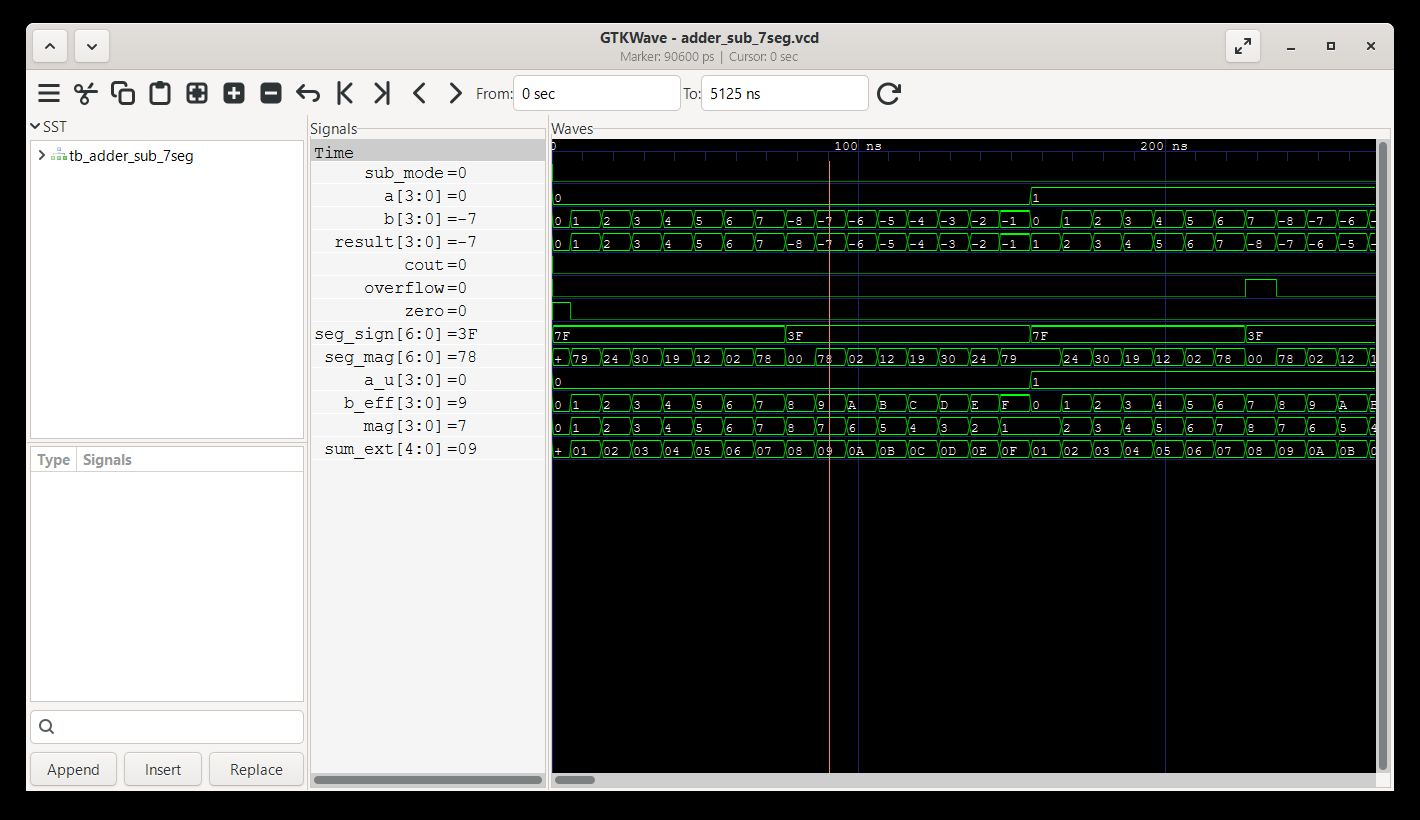
\includegraphics[width=0.95\textwidth,height=0.40\textheight,keepaspectratio]{figures/fig_0_gtkwave_waveform.png}
    \caption{GTKWave Verified Simulation Waveform (adder\_sub\_7seg) — 477 transition columns audited.}
\end{figure}

\begin{figure}[H]
    \centering
    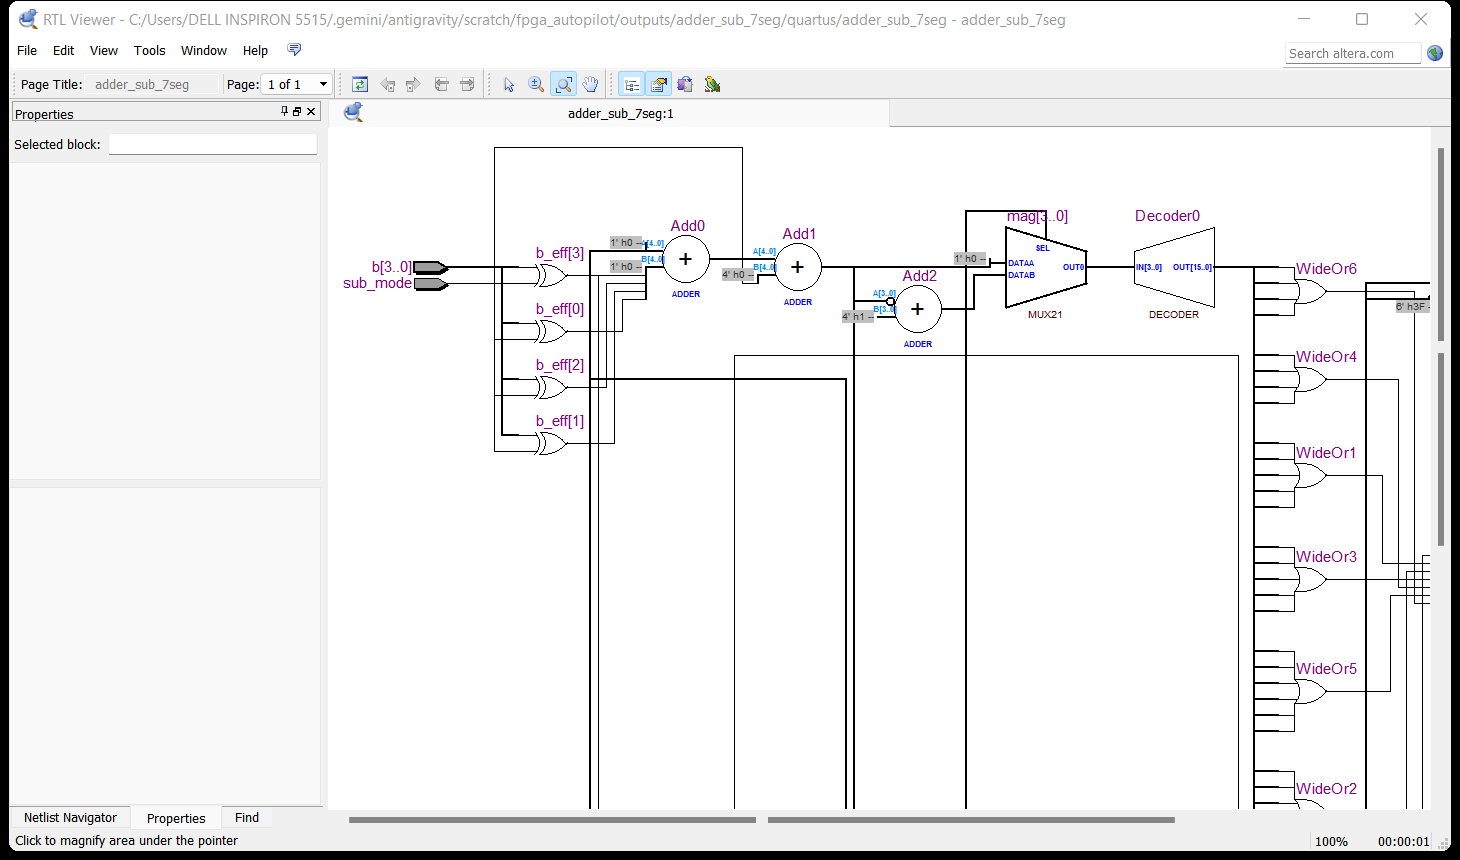
\includegraphics[width=0.95\textwidth,height=0.40\textheight,keepaspectratio]{figures/fig_1_quartus_rtl_viewer.png}
    \caption{Quartus II RTL Viewer Synthesized Schematic (adder\_sub\_7seg).}
\end{figure}


\end{document}
